\documentclass[black]{slideCEA}

\usetikzlibrary{decorations.text}
\usepackage{multicol}
%\usepackage{etoolbox}
\usepackage{mathrsfs}
%\usepackage{mathtools}
\usepackage[overload]{empheq}

\newcommand{\bOm}{\boldsymbol{\Omega}}
\DeclareMathAlphabet{\mathpzc}{OT1}{pzc}{m}{it}
\DeclareMathOperator{\sign}{sign}

%% %% Possible specific options:
%% %%   ** notofficial: change few aspect of the style: Front page, font black (not grey),
%% %%        !!! Compulsory to use the following two options
%% %%   ** topbar to get the path as ``section : subsection'' on top
%% %%   ** bottombar to get
%% %%          ==> left: date (with hidden link to toc if it exists, and its name is Menu, as here)
%% %%          ==> middle: subtitle (meeting name) - author
%% %%          ==> right: currentslidenb/totalslidenb (with hidden link to backup toc if it exists and is called MenuBackup, as here)
%% %%   Same links are hidden in official bottombar to avoid unpleasant scrolling
%% %%   CEA in official bottom bar can be changed to display institute like CEA/DIR/DEP/SER/LAB... with \BottomBarInstitute

%% %% Title of the slides and meeting
\YTitleFP{30}
\title{On the Ronen Method
       in simple 1D geometries}% \textcolor{white}{l}}
\FrontPageSubTitleY{55}
\subtitle{\textit{\normalsize Derivation of accurate expressions for the current in the slab and in the curvilinear reference frames}}
\date{September 27\textsuperscript{th}, 2019}
\Event{{\footnotesize 26\textsuperscript{th} International Conference on
       Transport Theory (ICTT26), Paris, France}}
\YEventFP{155}

%% %%%%%%%%%%%%%%%%%%%%%%%%%%%%%%%%%%%%%%%%%%%%%%%%%%%%%%%%%%%%%%%%%%%%%%%%%%
%% %%%%%%%%%%%%%% Personnal informations (most of which can %%%%%%%%%%%%%%%%%
%% %%%%%%%%% be put by default in the class file once and for all) %%%%%%%%%%
%% %%%%%%%%%%%%%%%%%%%%%%%%%%%%%%%%%%%%%%%%%%%%%%%%%%%%%%%%%%%%%%%%%%%%%%%%%%

%% %% Personnal information about the author
\YAuthFP{100}
%\author{Daniele Tomatis}
\author{Daniele Tomatis\\
        {\small \textcolor{ceared3}{CEA SERMA, France}
         \textcolor{blue}{(daniele.tomatis@cea.fr)}}}
%\MailAddress{daniele.tomatis@cea.fr}
%\Telephone{+33 (0)1 69 08 25 26}
%\Fax{(0)1 YY YY YY YY}
%% %% Possible option to add information on the author line (only for non-official for the moment)
\OtherAuthor{\\[6mm]Roy Gross and Erez Gilad\\[2pt]
             
\includegraphics[width=50mm]{logos/BGU_transp.png}
             % {\footnotesize University of Ben Gurion, Israel}
             }

%% %% Information about CEA: your service/departement/direction/centre
\Direction{Direction de l'{\'E}nergie Nucl{\'e}aire}
\Departement{D{\'e}partement de Mod{\'e}lisation des Syst{\`e}mes et Structures}
\Service{Service d'{\'e}tudes des r\'eacteurs et de math\'ematiques appliqu\'ees (SERMA)}
\Centre{Centre de Saclay}
\CentreAddress{91191 Gif-sur-Yvette Cedex, France}
\BottomBarInstitute{CEA/DEN/DANS/DM2S/SERMA/LPEC}

\CeaLogo{cea-tr.png}
%% %% On can change the logo with \CeaLogo{cea-saclay-tr.png} %% \CeaLogo{cea-den-tr.png}
%% %% One can add a picture in the Title bar of every slide. To do so, define
%% %% *** The path to the picture: \TitleBarPicture{Nobel-Prize-small.png}
%% %% *** The size of the picture (in mm): \TitleBarPictureSize{20} [20 is the default]
%% %% *** The X of the picture (in mm): \TitleBarPictureX{230} [230 is the default]
%% %% *** The Y of the picture (in mm): \TitleBarPictureY{0} [0 is the default]
%\TitleBarPicture{Nobel-Prize-small.png}
\TitleBarPicture{logos/BGU_transp_bk.png}
\TitleBarPictureSize{50}
\TitleBarPictureX{198}
\TitleBarPictureY{2}
\FrameTitleS{48}  % force line break in frametitle after 55 characters

\FrontPagePicture{logos/logo_ICTT26_white.png}
\FrontPagePictureX{10}
\FrontPagePictureY{90}
\FrontPagePictureSize{70}
%% %%%%%%%%%%%%%%%%%%%% Enf of personnal informations %%%%%%%%%%%%%%%%%%%%%%%

\graphicspath{{logos/}{../../../bgu_seminar/figures/}}

%% %% Starting the slide
\begin{document}

%% %% Front page (opening one)
\theframetitle

%% %% One can add a picture in the Front page. To do so, define
%% %% *** The path to the picture: \FrontPagePicture{Nobel-Prize-small.png}
%% %% *** The size of the picture (in mm): \FrontPagePictureSize{70} [70 is the default]
%% %% *** The X of the picture (in mm): \FrontPagePictureX{140} [140 is the default]
%% %% *** The Y of the picture (in mm): \FrontPagePictureY{70} [70 is the default]
%\FrontPagePicture{Nobel-Prize-small.png}
%\theframetitle

%% %%%%%%%%%%%%%%%%%%%%%%%%%%%%%%%%%%%%%%%%%%%%%%%%%%%%%%%%%%%%%%%%%%%%%%%%%%%%%
%% %% If none of the possible front page fit you, you can create your own doing
%% %% %%%%%%%%%%%% Or directly modify theframetitle in the class %%%%%%%%%%%%%%%
%% %%%%%%%%%%%%%%%%%%%%%%%%%%%%%%%%%%%%%%%%%%%%%%%%%%%%%%%%%%%%%%%%%%%%%%%%%%%%%
%% \begin{frame}[plain] %% begin frame
%%   \FrontPageRedStructure   %% add left bar with CEA logo and cea web address
%%   \begin{changemargin}{90 mm}{0cm} %% restraining the area to white space
%%     \begin{center}
%%       {\LARGE   \textcolor{ceared1}{Nouveau titre de présentation} }
%%     \end{center}
%%   \end{changemargin}
%% \end{frame}

%% the ``sections={1-\totvalue{SectionCounter}},'' comes along with usepackage{totcount}
%% It is used to get the section number of backup (if so) and not display it in this toc.
%% There is a specific toc for backup in \backupbegin
%% If one cannot install totcount, remove \tableofcontents[sections={1-\totvalue{SectionCounter}},

\setcounter{tocdepth}{2}
\setbeamertemplate{section in toc}[ball unnumbered]
\begin{frame}
  \frametitle{Outline}
%\begin{multicols}{2}
%\parbox[t]{.8\textwidth}{
\tableofcontents
%}
%\end{multicols}
\end{frame}


%\frame<4>[label=Menu]{
%  \frametitle{Sommaire}
%  \only<1>{\tableofcontents[sections={1-\totvalue{SectionCounter}},hideallsubsections]}
%  \only<2>{\tableofcontents[sections={1-\totvalue{SectionCounter}},currentsection,hideothersubsections]}
%  \only<3>{\tableofcontents[sections={1-\totvalue{SectionCounter}},currentsection,hideothersubsections,currentsubsection]}
%  \only<4>{\tableofcontents[sections={1-\totvalue{SectionCounter}},subsectionstyle=show]}
%}

\section{Introduction}

\begin{frame}
  \frametitle{Introduction and Motivation}
  \begin{itemize} \large
    \setlength{\itemsep}{5mm}
    \item The use of \textcolor{ceared1}{diffusion theory} is very practical in ordinary \textcolor{ceared1}{full core calculations} in terms of \emph{computational time} and \emph{numerical schemes}\\
    {\hfill \normalsize \color{ceagreen3}
    $\rightarrow$ fast calculations, parabolic/elliptic equations, diagonal dominance
    }
    % \pause
    \item Cross section preparation by \textcolor{ceared1}{homogenization} and \textcolor{ceared1}{equivalence} theory form a consistent frame-work with \textcolor{ceablue1}{nodal expansion} or \textcolor{ceablue1}{finite-element} solving methods\\
    {\hfill \normalsize \color{ceagreen3}
    $\rightarrow$ current standard approach in nuclear industry
    }
    % \pause
    \item Diffusion \textcolor{ceared1}{cannot} reproduce strong transport effects with sufficient accuracy\\%:

%   \begin{itemize} \large
%     \setlength{\itemsep}{3mm}
%     \item presence of void
%     \item regions of high absorption
%     \item materially heterogeneous systems
%     \item substantial scattering anisotropy
%   \end{itemize}

    {\hfill \normalsize \color{ceagreen3}
    $\rightarrow$ fails with strong absorption and flux gradients, rather miss anisotropy
    }
    \item {What's the \emph{best definition} of the diffusion coefficient? Is there any?}\\
    % \pause
    \item Influence of the {\color{ceared1}geometry frame} on the \emph{flux convergence} by Ronen iterations
  \end{itemize}
\end{frame}

%\begin{frame}
  \frametitle{Approaches to improve diffusion}

  \begin{block}{\bf Second-order transport approximations}
    {\vspace{3mm}
    \begin{itemize} \Large
      \setlength{\itemsep}{5mm}
      \item Different ``diffusive-like'' approximations of transport exist
      \item They can be implemented in existing diffusion-codes
    \end{itemize}
    }
  \end{block}
  \vfill
  \begin{exampleblock}{\bf \ldots{a} few examples:}
  {\vspace{3mm}
  \begin{itemize} \large
    \setlength{\itemsep}{5mm}
    \item \textcolor{ceablue1}{Diffusion tensors} to treat material heterogeneities with a \emph{drift component} \cite{boffi1972tensorial}
    \item Simplified $P_N$ or \textcolor{ceablue1}{$SP_N$} \cite{gelbard1960application, brantley2000simplified}, the \textcolor{ceablue1}{$A_N$} formulation \cite{PieroSNandAN, coppa2016an}
    \item \textcolor{ceablue1}{Quasi-diffusion} with the Eddington factor \cite{pounders2009diffusion}
    \item more accurate evaluation of the current in the actual system, i.e. the \textcolor{ceablue1}{Ronen Method} \cite{ronen2004accurate}
  \end{itemize}
  }
  \end{exampleblock}
\end{frame}

% ===================================

\section{Core Calculations}

% \subsection{Common features of core design}
% \begin{frame}
  \frametitle{Regularity, Periodicity and Modularity}
  \begin{columns}
  \vspace{-5mm}
    \column{0.425\linewidth}
    \begin{block}{}{ \sl
    ``A rich range of reactor types has been developed in years to accomplish various operating objectives and to overcome technological limitations, thus using different coolants and nuclear fuels''.}
    \end{block}
    %\vspace{5mm}
    %
    \begin{exampleblock}{}
    \begin{flushright}
      \textsc{LWR (PWR \& BWR), HWR, Gas-cooled and Graphite-moderated, LMFBR / SFR}, (+ \emph{research reactors}).
    \end{flushright}
    \end{exampleblock}
    \vspace{5mm}
    %
    \fbox{\parbox{\textwidth}{ \centering
    Homogeneous~vs.~\emph{Heterogeneous systems}\\
    $\implies$ higher resonance escape probability.
    }}\vspace{5mm}
    %
    \begin{block}{\sl Features of the active core geometry}
      \textcolor{ceared1}{lattice} (\emph{regularity}) and \textcolor{ceared1}{assemblies} (\emph{modularity}), \emph{periodically} filling the multiplying system to achieve the target power.
    \end{block}
    %
    \column{0.575\linewidth} \centering
    {
    Hierarchical structure of a water reactor (PWR top, BWR bottom).}\\
    \includegraphics[width=0.8\textwidth]{figures/HierarcicalStructurePWR.png}\\[2mm]
    \includegraphics[width=0.8\textwidth]{figures/bwr_bundle.jpeg}
  \end{columns}
\end{frame}


\subsection{Two-step calculation scheme}
\begin{frame}
  \frametitle{Two-step core calculations}

  \begin{columns}
  \vspace{-5mm}
    \column{0.65\linewidth} \centering
    {\includegraphics[width=\textwidth]{FA_homog.png}}
    \column{0.35\linewidth} \centering
    {\includegraphics[width=0.9\textwidth]{core_quarter.png}}
  \end{columns}

  \begin{tikzpicture}[overlay, remember picture]
  \draw[->, thick, draw=ceagreen2, line width=5mm]
    ([yshift=3cm, xshift=-2cm]current page.south)
    -- ([yshift=3cm, xshift=-8.5cm]current page.south east)
    node[midway, above] {\color{ceagreen3}\large \tt \bf
    \begin{tabular}{c}
    multi-group \\ xs library
    \end{tabular}
    };
%    [xshift=-2cm, yshift=2cm]
  \end{tikzpicture}
\end{frame}

%%% this does not work %%%
%\begin{frame}
%  \frametitle{3D Coarse Mesh Kinetics}
%  \label{sec:fm3D}
%  \input{coarse_mesh3D}
%\end{frame}

\subsection{Transport effects in core calculations}
\begin{frame}
  \frametitle{\insertsubsectionhead}
  \begin{block}{General issues for safety and design calculations}% or warnings?
  { \vspace{3mm}
  %
  \begin{itemize} \large
    \setlength{\itemsep}{3mm}
    \item \textcolor{ceablue1}{High absorption} and \textcolor{ceablue1}{low scattering}: presence of black materials to neutrons (mechanical and chemical shim), weak moderation, spectrum hardening
    %\item \textcolor{ceablue1}{high absorption}, like with the elements close to the thermal energy range causing neutron spectrum hardening (mechanical shim by black control rods, fuel blended with burnable poisons)
    \item \textcolor{ceablue1}{scattering anisotropy}: e.g. forward-peaked moderation in water
    \item potential \textcolor{ceablue1}{occurrence of void} under operation or in accidental transients (LWR/FR)
    \item angle-dependent boundary conditions: free-surfaces-vacuum, anisotropic albedos
    \item \textcolor{ceablue1}{steep flux gradients}: proximity to the reflector in thermal reactor, strong localized absorption
    %\item boundary with selective and anisotropic reflection (e.g. heavy reflector to extend the vessel lifetime or the respose of water reflector in fast groups)
    \item \textcolor{ceablue1}{material heterogeneity}: heterogeneous core loading with material discontinuities at the interfaces between fuel elements (MOX/UO2 mixed cores, with both radial and axial discontinuities)
    \item \emph{memory-effects} due to temporary and localized short reactivity insertion (incore instrumentation, rapid geometry and material changes, presence of noise)
  \end{itemize}
  }
  \end{block}
\end{frame}
% ===================================

\section{Diffusion Theory}

\subsection{Conservation equation and Fick's law}
\begin{frame}
  \frametitle{Continuity equation with approximated transport law}
  %
  \vspace{-5mm}
  \begin{block}{Integro-differential Neutron Transport Equation (NTE)}
  {\hfill \normalsize \cite{duderstadt1979transport}}
  {
  \begin{gather*}
  \left[ \frac{1}{v}\frac{\partial}{\partial t}
  %+ \nabla \cdot (\bOm \,\_) + \Sigma_t(\mathbf{r}, E) \right] \varphi(\mathbf{r}, E, \bOm)
  + \bOm \cdot \nabla + \Sigma_t(\mathbf{r}, E) \right] \varphi(\mathbf{r}, E, \bOm, t)
  = \frac{\chi(E)}{4\pi} \int_0^{\infty} {dE' \nu\Sigma_f(\mathbf{r}, E') \phi(\mathbf{r}, E', t)}
  + s_{\text{ext}}(\mathbf{r}, E, \bOm, t) +\\
  \int_{4\pi} d\bOm'
  \int_0^{\infty} {dE' \Sigma_s(\mathbf{r}, E' \rightarrow E, \bOm' \rightarrow \bOm)
  \varphi(\mathbf{r}, E', \bOm', t)
  } = q(\mathbf{r}, E, \bOm, t).
  \end{gather*}
  }
  \end{block}
  Let us introduce the scalar flux and the current, respectively:
  \[
    \phi = \int_{4\pi}{d \boldsymbol{\Omega}
    \varphi(\mathbf{r}, \boldsymbol{\Omega}[, \ast] )}
    \quad \text{and} \quad
    \mathbf{J} = \int_{4\pi}{d \boldsymbol{\Omega} \boldsymbol{\Omega}
    \varphi(\mathbf{r}, \boldsymbol{\Omega}[, \ast] )},
  \]
  and integrate the NTE to get the continuity equation:
  \[
    \frac{1}{v}\frac{\partial \phi}{\partial t} + \nabla \cdot \mathbf{J}
    + \Sigma_t \phi = \int_{4\pi}{d \bOm \, q(\mathbf{r}, \boldsymbol{\Omega}[, \ast] )}.
  \]
  Use \textcolor{ceared1}{Fick's law} as closure
  \textcolor{ceared1}{$\mathbf{J} = - \mathcal{D}\nabla \phi$}, with the
  vacuum bnd. conds. $- \partial_{\hat{n}} \phi = \phi/
  \zeta$ and the extrapolated length $\zeta = 2\mathcal{D}$ ($\approx 2.13
  \mathcal{D}$ in computer codes).
  \begin{alertblock}{}
    \textit{N.B. A unique family of fissiles is represented here;
    precursors of delayed neutrons are also necessary for kinetics
    with fission; $\Sigma_t(\bOm[, \ast])$ if no rotational symmetry
    in scattering events.}
  \end{alertblock}
\end{frame}

% WARNING: it is important to remind that the source term in the trasnport
% equation is given as sum of moments on spherical harmonics!
% \begin{frame}
  \frametitle{Treatment of scattering anisotropy as in ENDF}
  \begin{block}{Introducing the flux moments on spherical harmonics in the NTE}
  {
  \begin{gather*}
  \left[ \frac{1}{v}\frac{\partial}{\partial t}
  %+ \nabla \cdot (\bOm \,\_) + \Sigma_t(\mathbf{r}, E) \right] \varphi(\mathbf{r}, E, \bOm, t)
  + \bOm \cdot \nabla  + \Sigma_t(\mathbf{r}, E) \right] \varphi(\mathbf{r}, E, \bOm, t)
  = \frac{\chi(E)}{4\pi} \int_0^{\infty} {dE' \nu\Sigma_f(\mathbf{r}, E') \phi(\mathbf{r}, E, t')}
  + S_{ext}(\mathbf{r}, E, \bOm, t) +\\
  \visible<2-3> {\frac{1}{2\pi}}
  \only<-3>{\int_{4\pi} d\bOm'}
  \only<4->{ \sum_{\ell = 0}^{\infty} \sum_{m=-\ell}^{\ell}  Y_{\ell m}(\bOm) }
  \int_0^{\infty} {dE' \only<-3>{\Sigma_s}\only<4->{\Sigma_{s, \ell}}
  (\mathbf{r}, E' \rightarrow E
  \only<1> {, \bOm' \rightarrow \bOm)}
  \only<2-3>{, \textcolor{ceablue1}{\bOm' \cdot \bOm})}
  \only<-3>{\varphi(\mathbf{r}, E', \bOm', t)}
  \only<4->{)\phi_{\ell m}(\mathbf{r}, E', t) }
  },
  \end{gather*}
  }
  {\sl hp.}: a unique family of fissile nuclides, all prompts -- b.c. at $\mathbf{r}_S$: $\varphi(\mathbf{r}_S, E, \bOm) = 0$ if $\hat{n} \cdot \bOm < 0$, $\forall E$. \uncover<2->{$\mu_0 = \bOm \cdot \bOm'$ is the cosine of the scattering angle.} \uncover<3->{Thanks to the addition theorem $P_0$ is written in terms of the spherical harmonics functions $Y_{\ell m}$}
  \uncover<2->{ \[
    \Sigma_s(\mathbf{r}, E' \rightarrow E, \mu_0) = \sum_{\ell = 0}^{\infty}{\frac{2\ell + 1}{2}\Sigma_{s,\ell}(\mathbf{r}, E' \rightarrow E) P_\ell(\mu_0)}
   \visible<3-> {= 2\pi \sum_{\ell = 0}^{\infty} {\sum_{m=-\ell}^{\ell}{ \Sigma_{s,\ell} Y^*_{\ell m}(\bOm') Y_{\ell m}(\bOm)}}}
  \]}
  \uncover<3->{\emph{Spherical harmonics} in $\bOm = (\mu, \theta)$, defined by associated Legendre polynomials $P_{\ell}^m$:
  \[ Y_{\ell m}(\bOm) = \left[ \frac{2 \ell+1}{4\pi} \frac{(\ell - |m|)!}{(\ell + |m|)!} \right]^{1/2} P_{\ell}^m (\mu)e^{i m \theta}
  \uncover<4->{ \quad
  \text{so that } \textcolor{ceablue1}{
  \varphi = \sum_{\ell = 0}^{\infty} \sum_{m=-\ell}^{\ell} \left( \frac{2\ell + 1}{4\pi} \right)^{1/2} \phi_{\ell m}(\mathbf{r}[, \ast]) Y_{\ell m}(\bOm)}}
  \]
  and subject to the orthogonal-normalization property $\int_{4\pi} {d \bOm Y^*_{\ell m}(\bOm) Y_{k n}(\bOm)} = \delta_{\ell k}\delta_{m n}$.}
  \end{block}
\end{frame}



\subsection{About the diffusion coefficient}
%
\begin{frame}%[t] \vspace{5mm}
  \frametitle{The $P_1$ branding of the diffusion coefficient}
  \begin{alertblock}{} \large
  $P_N$: flux expansion on sph. harmonics and projections over $4\pi$ of the NTE on $1$, $\bOm$, $\ldots$
  \end{alertblock}
  \begin{block}{If we limit the expansion to the first moment:}
  {
  %\[ \left\{
  \begin{align}[left=\empheqlbrace]
  \frac{1}{v} \frac{\partial \phi}{\partial t} + \nabla \cdot \mathbf{J} + \Sigma_t\, \phi &=
  \int_0^{\infty} {dE' \Sigma_{s,\ell=0}(E' \rightarrow E)\,\phi(\mathbf{r}, E', t) \ }
  + S_{\text{ext},\ell = 0},\label{eq:sflx}\\[3mm]
  \frac{1}{v} \frac{\partial \mathbf{J}}{\partial t} + \nabla \cdot \boldsymbol{\Pi} + \Sigma_t\, \mathbf{J} &= \int_0^{\infty} {dE' \Sigma_{s,\ell=1}(E' \rightarrow E)\, \mathbf{J}(\mathbf{r}, E', t)} + \mathbf{S}_{\text{ext},\ell = 1},\label{eq:curr}
  \end{align}
  %\right. \]
  }\vspace{5mm}
  with $\boldsymbol{\Pi} = \int_{4\pi}{d \bOm (\bOm \bOm)\varphi(\mathbf{r}, \bOm}[, \ast])$,
  or \textcolor{ceablue1}{$\boldsymbol{\Pi} = \phi / 3$} if
  \textcolor{ceablue1}{$\varphi = \left( \phi + 3 \mathbf{J} \cdot \bOm \right)/4\pi$},
  i.e. the \textcolor{ceared1}{$P_1$ approximation}.\vspace{5mm}

  \pause{
  Use then the \textcolor{ceablue1}{multi-group energy formalism} in Eq. \ref{eq:curr}, assume \textcolor{ceablue1}{stationarity} and an \textcolor{ceablue1}{isotropic external source} to write:
  \[
  \frac{1}{3}\nabla \phi_g + \Sigma_{t,g} \,\mathbf{J}_g = \sum_{g'=1}^G {\Sigma_{s,1,g' \rightarrow g}\, \mathbf{J}_{g'}}
  \]
  }\vspace{5mm}

  \pause{
  In presence of dominant scattering and at \emph{thermal equilibrium} \textcolor{ceagreen3}{$\sum_{g'} {\Sigma_{s,1,g' \rightarrow g} \mathbf{J}_{g'}} \approx \mathbf{J}_{g} \sum_{g'} {\Sigma_{s,1,g \rightarrow g'}}$}, thus yielding a specific diffusion coefficient:
  \[
  \mathbf{J}_g = -D_g \nabla \phi_g \implies
    \textcolor{ceared1}{D_g(\mathbf{r}) = \frac{1}{3\Sigma_{tr,g}}}
    \quad \text{with} \quad \Sigma_{tr,g} = \Sigma_{t,g} - \Sigma_{s,1,g}, \; \forall g.
  \]
  }
  \end{block}
\end{frame}

% \begin{frame}
  \frametitle{Other diffusive-like approximations from radiative transfer problems}
  \begin{block}{Flux-limited diffusion}
  {
  The angular flux is factored in a term slowly varying in space and a normalized angular component \cite{levermore1981flux}:
  \[
  \varphi \approx \phi(\mathbf{r}, E) \psi(\mathbf{r}, \bOm) \quad \text{with} \quad \int_{4\pi} {d \bOm \psi} = 1,
  \quad \implies \mathbf{J}_g = \mathbf{f}(\mathbf{r})\,\phi_g \; \wedge \;
  \frac{\lVert \mathbf{J}_g \rVert}{\phi_g} = \text{const},\; \forall g.
  \]
  The diffusion coefficient (``the flux-limiting parameter'') come from the solution of a \emph{transcendental equation}. In the limit of weak gradients, the diffusion coefficient is obtained as (for all groups):
  \[ \textcolor{ceared1}{
  D_g(\mathbf{r}) = \frac{1}{3} \left[ \Sigma_{t,g} - \sum_{g'}{\Sigma_{s,1,g' \rightarrow g} \,\frac{\phi_{g'}}{\phi_g}} \right]^{-1}}
  \]
  }
  \end{block}
  %
  \begin{block}{Variable Eddington factor}
  {
  Postulate a factorization of the second moment by another factor (or \emph{tensor}) slowly varying in space \cite{pomraning1982flux}:
  \[
  \varphi \approx E(\mathbf{r}[, \ast]) \phi(\mathbf{r}[, \ast]),
  \text{ and }
  \partial_{\mathbf{r}} E \approx 0 \hfill \implies
  \textcolor{ceared1}{
  D_{i,g}(\mathbf{r}) = E_g(\mathbf{r}) \left[ \Sigma_{t,g} - \sum_{g'}{\Sigma_{s,1,g' \rightarrow g} \,\frac{J_{i,g'}}{J_{i,g}}} \right]^{-1}, i \in (\hat{e}_x, \hat{e}_y, \hat{e}_z).}
  \]
  }
  \end{block}
\end{frame}


% \subsection{The fundamental leakage model}
% \begin{frame}
  \frametitle{The $B_N$ leakage model}
  \begin{alertblock}{Objective}
    Get a critical flux by adjusting the leakage in each group, and obtain a consistent definition of the diffusion coefficient \cite{benoist1964theorie, hebert2009applied}.
  \end{alertblock}
  %
  \begin{block}{Assumptions}
  {
  \begin{itemize} \normalsize
    \item Closed system by \emph{reflective} or \emph{periodic} bnd. conds. in a \textcolor{ceagreen1}{finite lattice of cells or assemblies}.
    \item Flux factorization with a \emph{macroscopic} quantity $\phi$ and a \emph{homogeneous} or \emph{periodic} \textcolor{ceablue1}{fundamental flux} $\psi$, \[\textcolor{ceared1}{\varphi(\mathbf{r}[, \ast]) = \phi(\mathbf{r})\, \psi(\mathbf{r}[, \ast])},\] where $\phi$ fulfills the Helmholtz eqn. $\nabla^2 \phi + B^2 \phi = 0$ with the (\underline{critical}) buckling $B^2 \in \mathbb{R}$. It follows that $\phi \propto \exp(i \mathbf{B} \cdot \mathbf{r})\; (B^2 = \mathbf{B} \cdot \mathbf{B})$.
    \item homogeneous or heterogeneous variants (acc. to the dependence of $\psi$ on $\mathbf{r}$)
  \end{itemize}
  }
  \end{block}
  %
  \begin{exampleblock}{Homogeneous $B_1$ Equations}
  {
  After a flux-volume homogenization of the NTE, substitute $\varphi = \psi(E, \bOm)\exp(i \mathbf{B} \cdot \mathbf{r})$ and integrate on angle to obtain the system of eqs. (with $\gamma$ as polynomial function of $(B/\Sigma_t)^2$):
  %\[ \left\{ \begin{split}
  \begin{align*}[left=\empheqlbrace]
    (\Sigma_t(E) + D(B, E)B^2) \psi(E) = \int_{0}^{\infty}{dE' \left(\Sigma_{s,0}(E' \rightarrow E) + \chi(E) \nu\Sigma_f(E') \right)\psi(E')}\\
    \textcolor{ceared1}{
    D(B, E) = \frac{1}{3\gamma(B, \Sigma_t)\Sigma_t}\left[ 1 + 3\int_{0}^{\infty} {dE' \Sigma_{s,1}(E' \rightarrow E) D(B, E') \frac{\psi(E')}{\psi(E)}} \right]}
  \end{align*}
  %\end{split} \right. \]
  }
  \end{exampleblock}
\end{frame}


\subsection{Diffusion tensors}
\begin{frame}
  \frametitle{Drift, diffusion tensors, and more$\ldots$}
  %
  \begin{block}{Integral Neutron Transport Equation}
   \begin{gather*}
   \varphi({\mathbf{r}, E, \bOm}) =
     \int_0^{\mathpzc{S}(\mathbf{r},\bOm)}{ds\,
     q(\mathbf{r} - s\, \bOm, E, \bOm) \exp{ \left[
     - \mathscr{L}_{op}(\mathbf{r}, s, E, \bOm) \right]}
   }\text{ with } \mathscr{L}_{op} = \int_0^{s}{ds'\, \Sigma_t(\mathbf{r} - s'\, \bOm, E)},\\
     q(\mathbf{r}', E, \bOm) = \sum_{\ell m} {Y_{\ell m}(\bOm)
       \int_0^{\infty}{dE' \left( \Sigma_{s,\ell}(\mathbf{r}', E' \rightarrow E)
       + \chi(E) \nu\Sigma_f(\mathbf{r}', E')\delta_{\ell 0}\delta_{m 0} \right)
       \phi_\ell^m(\mathbf{r}', E')}} + \text{b.c.}
   \end{gather*}

  \end{block}
  %
  \begin{columns}
  \column{.325\textwidth}
  \def\dx{0.25}
  \begin{tikzpicture}[declare function={f(\x) = (\x - 1)/3+2;}]
   \draw[->, very thick] (1,0) -- (4,{f(4)}) node[below right] {
     \begin{tabular}{c}
       $\mathbf{r}' = \mathbf{r}-s\, \bOm$,\\
       $s = \lVert \mathbf{r}' - \mathbf{r} \rVert$
     \end{tabular}
   };
   \draw[->, very thick] (0,0) -- (1,{f(1)}) node[below right] {$\mathbf{r}$};
   \draw[->, thick] ({4-\dx},{f(4)+\dx}) -- ({3-\dx},{f(3)+\dx}) node[above left] {$s, \bOm$};
   \draw[->,dashed] (0,{f(0)}) -- (1,{f(1)}) -- (4,{f(4)}) -- (5.5,{f(5.5)})
     node[above right] {$\mathpzc{S}$};
   \draw[ultra thick] plot[smooth] coordinates {(3,4) (5.5,{f(5.5)}) (6,3)};
  \end{tikzpicture}
  %
  \column{.675\textwidth}
  \begin{block}{}
  {Assume \textcolor{ceared1}{isotropic} sources (with pure scattering and one group for simplicity), expand the flux by Taylor around $\mathbf{r}$ and integrate to obtain the current:
  \begin{flalign*}
  \begin{split}
  %\mathbf{J}(\mathbf{r}) = \frac{1}{4\pi}
  %  \int{ d \bOm \int_0^{\mathpzc{S}}{
  %    ds\,\bOm\, \Sigma_{s,0}(\ast) \exp\left[ \mathscr{L}_{op} \right] \cdot\\
  %    \left( \phi(\mathbf{r}) - \bOm \cdot \nabla \phi \,s
  %           + \bOm \mathbf{H} \bOm\, s^2 + O(s^3)\right)
  %    }}
  \mathbf{J}(\mathbf{r}) = \int d\mathbf{r}'
    \frac{\mathbf{r}' - \mathbf{r}}
         {4\pi \lVert \mathbf{r}' - \mathbf{r} \rVert^3}
      \Sigma_{s,0}(\ast) e^{ -\mathscr{L}_{op} } \cdot \\
      \left( \phi(\mathbf{r}) - s \, \bOm \cdot \nabla \phi
             + s^2 \, \bOm \mathbf{H} \bOm + O(s^3)\right)\\[3mm]
    \Rightarrow \textcolor{ceared1}{
    \mathbf{J}(\mathbf{r}, E) =
      \underbrace{\vec{\mathpzc{d}}(\mathbf{r}, E) \phi(\mathbf{r}, E)}_\text{
      advection~/~drift}
      - \underbrace{\mathbf{D}(\mathbf{r}, E) \nabla \phi(\mathbf{r}, E)}_\text{
      term w. diffusion tensor}
      + \ldots
    }
  \end{split}
  \end{flalign*}
  }
  \end{block}
  \end{columns}
  %
  \begin{columns}
  \column{.6\textwidth}
  \begin{exampleblock}{Under the following conditions:}
  \begin{enumerate}[i.]
    \item smooth flux gradient and small higher derivatives
    \item weakly absorbing and highly scattering media
    \item \textcolor{ceablue1}{constant cross sections in space}
  \end{enumerate}
  \end{exampleblock}
  %
  \column{.4\textwidth}
  \[ \Rightarrow \textcolor{ceared1}{
    \mathbf{J} = -D \nabla \phi \quad \text{with}
    \quad D = \frac{\Sigma_s}{3 \Sigma_t^2}
  }\]
  \end{columns}
\end{frame}
% ===================================

% \section{Cross section preparation}
% \subsection{Homogenization and Equivalence Theory}
% \begin{frame}
  \frametitle{Homogenization and Equivalence Theory}
  %
  \begin{block}{} \begin{flushright}
  \textcolor{ceared1}{\Large What for?} Prepare \emph{in advance} all reactor data for later core calculations in \textcolor{ceablue1}{low-order transport} (diffusion, $SP_N$ and others). \end{flushright}
  \end{block}\vspace{5mm}
  %
  \begin{alertblock}{Main rational of Homogenization}
    Conservation of reaction rates in the volume $\mathcal{V}$ of
    \emph{spatial homogenization} and
    in the $g$-th group of \emph{energy condensation} with
    $E \in [E_g, E_{g+1}]$, $g = 1, \ldots, G$.
  \end{alertblock}
  %
  \[
  \Sigma_g = \frac{\displaystyle
    \int_{\mathcal{V}} d\mathbf{r} \int_{E_{g+1}}^{E_g} dE \,
      \Sigma(\mathbf{r}, E) \, \phi(\mathbf{r}, E) }{\displaystyle
    \int_{\mathcal{V}} d\mathbf{r} \int_{E_{g+1}}^{E_g} dE \, \phi(\mathbf{r}, E)
    } \quad \text{with} \quad \chi_g = \int_{E_{g+1}}^{E_g} dE \, \chi(E).
  \]
  %
  \begin{columns}
    \column{.6\textwidth}
      \begin{block}{Equivalence}
      \textcolor{ceared1}{\Large Why?} $\ldots$Diffusion $\not\equiv$ transport, conservation of reaction rates does not imply to reproduce the \emph{same currents} at the boundaries of $\mathcal{V}$. Available techniques:
      \begin{itemize}
        \item (A)DF$ = \phi_{\text{het}}/\phi_{\text{hom}} $ (discontinuity factors), \emph{two per direction}
        \item SPH (SuPer-Homogenization) factors, \emph{one per group and homog. region}: $(\Sigma^{(k)}_g / s)(s\phi^{(k)}_g)$
      \end{itemize}
    \end{block}
    %
    \column{.4\textwidth} \centering
    \def\wdt{2.5}
    \def\ymin{0.25}
    \begin{tikzpicture}
      \draw[->, thin, help lines] ({-\wdt-0.5},{\ymin+0.1})
        -- ({\wdt+1},{\ymin+0.1}) node[right] {$\hat{e}_k$};
      \draw[-] (-\wdt,\ymin) node[below] {$k-1/2$} -- (-\wdt,3);
      \draw[-] ({\wdt-1/4},\ymin) node[below] {$k+1/2$} -- ({\wdt-1/4},3);
      \draw[->] ({-\wdt-0.5}, 2.4) -- ({-\wdt-0.1}, 2.4)
        node[midway,above] {$J^+_{\text{in}}$};
      \draw[black, domain={-\wdt}:{\wdt-1/4}]
        plot[samples=100]
        ({\x}, {2+0.2*sin(((\x+2)*4)*3.141592 r)-0.2*\x})
        node[right] {$\phi_{\text{het}}$};
      \draw[red, domain={-\wdt}:{\wdt-1/4}, thick]
        plot[samples=100] ({\x}, {0.5+exp(-0.35*\x)})
        node[right] {$\phi_{\text{hom}}$};
      \node[red,below] (D) at (\ymin,1.35) {$D^{(k)}$};
      \node (title) at (0,3) {$k$'th cell};
    \end{tikzpicture}
  \end{columns}
\end{frame}

% ===================================

\section{The Ronen Method}

\subsection{Principles \& Implementation}
%
\begin{frame}
  \frametitle{\insertsectionhead}
  \begin{block}{Principles \& Implementation}
  {\hfill \cite{ronen2004accurate, tomatis2011application}}
  {
  \begin{itemize} \large
    \setlength{\itemsep}{3mm}
    \item The \textcolor{ceared1}{best diffusion coefficient} would be the one satisfying exactly Fick's law with the same flux and current computed by transport (with the current containing all contributions from higher order moments!)
    \item<2-> Use a higher-order \textcolor{ceablue1}{integral} transport operator to obtain \textcolor{ceared1}{more accurate estimates of the current} \emph{by sources determined with the diffusion flux}
    % \item<2-> An ``\textcolor{ceared1}{equivalent}'' (\textcolor{ceablue1}{integral}) transport problem is defined to determine the diffusion coefficient:
    % \[
    %  D_i = - \frac{\mathbf{J} \cdot \hat{e}_i}
    %    {\nabla \phi \cdot \hat{e}_i},
    %  \text{ where \textcolor{ceared1}{$\mathbf{J}$ is estimated by a higher order transport operator!}}
    % \]
    \item<3-> Solve diffusion \emph{again} with the new coefficients $D_i = - \left[\mathbf{J}(\phi) \cdot \hat{e}_i\right] \big/ \left[ \nabla \phi \cdot \hat{e}_i\right]$
    \item<4-> Such agreement is sought numerically by \textcolor{ceablue1}{non-linear iterations}
    \item<5-> \textcolor{ceared1}{Alternative implementation} by a CMFD-like scheme \cite{smith1983nodal}, with currents at cell interfaces as:
    \[
    J^{(k,+)} \approx
    \underbrace{
    - 2D_\text{DIFF} \frac{\phi^{(k+1,+)} - \phi^{(k,+)}}{\Delta_{k+1} + \Delta_{k}}
    }_\text{Diffusive current}
    -2 \underbrace{
    (\textcolor{ceared1}{\delta D})
      \frac{\phi^{(k+1,+)} \textcolor{ceared1}{+} \phi^{(k,+)}}{\Delta_{k+1} + \Delta_{k}}
    }_\text{Transport correction},
    \]
    where $\textcolor{ceared1}{\delta D} \propto (J_{\text{TRANSP}} - J_\text{DIFF})$.
  \end{itemize}
  }
  \end{block}
\end{frame}

\begin{frame}
  \frametitle{Boundary conditions (bc.)}

  \begin{alertblock}{A known issue\ldots}
    bc. apply on the angular flux in transport and we solve only for the scalar flux in diffusion.
  \end{alertblock}
  { Generalized form for finite difference equations:
  \[
    J = - \frac{D \phi_{bc}}{\Delta_{bc} / 2 + \zeta} \text{ with }
    \begin{cases}
      \zeta \propto \lambda_t & \text{extrapolated length for vacuum}, \\
      \zeta = 0 & \text{zero flux}, \\
      \zeta \rightarrow 0^+ & \text{reflection by vanishing current};
    \end{cases} \qquad \delta J_{bc} = \delta D \phi_{bc}.
  \]
  }\vspace{-10mm}

  \visible<2->{
    \flushright \textcolor{ceared1}{\large bc. are given for incoming
    particles\\and we use a transport operator to estimate the current!}\\[3mm]
  }

  \begin{block}{The problem of reflection and periodic translation}
    We expand the angular flux on spherical harmonics to get expressions based
    on moments. Now consider a bare homogeneous slab
    ($\varphi \approx \phi/2 + 3/2 J \mu$) with specular reflection at one side.
    \alert<3>{$J^+ + J^- \neq 0$} at the refl. boundary for $\varphi \approx \phi/2$.
    {
      $\longrightarrow$ Fix $J=0$ by corrections from higher moments as:
      \begin{equation*}
      \begin{split}
      J^+(x) &= \frac{\phi_0(a)}{2}E_3(\tau(a, x)) + \frac{5}{4} \tilde{\phi}_2(a) \left[ 3 E_5(\tau(a, x)) - E_3(\tau(a, x)) \right],\\
             \text{with }& \tilde{\phi}_2(a) = - \frac{16}{5} \left( \frac{1}{4} \phi_0(a) + J^- \right) \text{ and }
      \phi(a, \mu) = \frac{1}{2} \phi_0 + \frac{3}{2} \mu \phi_1 + \frac{5}{4} \left( 3 \mu^2 - 1 \right) \tilde{\phi}_2.
      \end{split}
      \end{equation*}
    }
  \end{block}
\end{frame}

\subsection{Expressions for the current in simple 1D geometries}

\begin{frame}
  \frametitle{Expressions for the current in simple 1D geometries}

  \vspace{-5mm}
  {Derivation of the equation for the current in mono-dimensional problems
  (\emph{bare bodies}) by \textcolor{ceared1}{escape probabilities}.
  The current of particles crossing the surface $S$ at $r$ is
  \[
    J(r) S(r) = \sum_j q_j V_j e_{j}(r), \text{ where}
  \] \vspace{-5mm}
  \begin{itemize}
    \item $q_j$ is the (isotropic) source in the region $j$ of volume $V_j$ and\\
    \item $e_j(r)$ is the probability for a particle isotropically emitted
          in region $j$ to cross S(r) uncollided.
  \end{itemize}
  }
  \begin{figure}[t]
    \centering
    \scalebox{1.5}{
      \input{../figures/mesh1d.tkz}
    }
    \caption{Mesh notation for the 1d problems.}
  \end{figure}
  {
  In \textcolor{ceablue1}{\bf 1D slab}, integration on the polar angle is resolved \emph{analytically} by \textcolor{ceablue1}{exponential integral functions $E_n$}:
  % \[
  %   E_n(\tau) = \int_1^{\infty}{du\, \frac{e^{-|tau|\,u}}{u^n}}
  %     = \int_0^1 {d\mu \, \mu^{n-2} e^{-|\tau| / \mu}}.
  % \]

  \begin{equation*}
  \begin{split}
  J_{i+1/2} =& \int_0^1   {d\mu\, \mu \varphi(a, \mu) e^{-\tau(a, x_{i+1/2})/\mu}}
             - \int_0^{-1}{d\mu\, \mu \varphi(b, \mu) e^{-\tau(b, x_{i+1/2})/\mu}}\\
          +& \sum_{j=0}^{I-1} { \sign(x_{i+1/2} - x_{j+1/2}) \frac{q_{0,j}}{2} \int_{x_{j-1/2}}^{x_{j+1/2}}{dx'
          E_{2} \left(\lvert \tau(x', x_{i+1/2}) \rvert \right) } }.
  \end{split}
  % \label{eq:J_tr}
  \end{equation*}
  }
\end{frame}


\subsubsection{Slab}

\begin{frame}[allowframebreaks]
  \frametitle{An example in the bare homogeneous slab}
  {\hfill \cite{tomatis2011application}}%\\[3mm]

  \begin{block}{}
  % In 1-D, we find the \textcolor{ceablue1}{exponential integral functions $E_n$} and the diffusion tensor simplifies in a single coefficient.
  % \[
  %   \begin{split}
  %   E_n(\mathcal{L}_{op}) = \int_1^{\infty}{du\, \frac{e^{-|\mathcal{L}_{op}|\,u}}{u^n}}\\
  %     = \int_0^1 {d\mu \, \mu^{n-2} e^{-|\mathcal{L}_{op}| / \mu}}.
  %   \end{split}
  % \]
  {\textcolor{ceablue1}{APPROX}: 2G problem with isotropic scattering, extrapolated length $\zeta = 2.13 \mathcal{D}$}\\
  {\textcolor{ceablue1}{b.c.}: reflection at left, vacuum or zero flux at right.}
  \end{block}

  \begin{table}
  \centering
  \caption{Cross section data of the homogenized FA ($k_{\infty} = 1.07838$); scattering cross section comes from sum on columns.}
  \begin{tabular}{*{6}{c}}\hline \hline
  Group $g$ & $\Sigma_{t,g}$ & \multicolumn{2}{c}{$\Sigma_{s,0,g' \rightarrow g}$} &
  $\chi_g$ & $\nu\Sigma_f$ \\ \hline
  1 & 5.31150E-01 & 5.04664E-01 & 2.03884E-03 & 1 & 7.15848E-03 \\
  2 & 1.30058E+00 & 1.62955E-02 & 1.19134E+00 & 0 & 1.41284E-01 \\
  \hline \hline
  \end{tabular}
  \end{table}

  \begin{columns}
  \column{.5\textwidth}
  \begin{table}\centering
  \caption{17$\times$17 PWR UO2 FA data (3.5\% enr. w/o $^{235}$U).}
  \begin{tabular}{lc} \hline \hline
    Slab width & 21.5 cm\\
    Fuel temp. & 900 K\\
    Water temp.& 600 K\\
    Water density& 0.66 g/cm$^3$\\
    Boron conc.& 500 ppm\\ \hline \hline
  \end{tabular}
  \end{table}
  \column{.5\textwidth}
  \begin{table}
  \centering
  \caption{Results on the multiplication factor $k$}
  \begin{tabular}{*{4}{c}} \hline \hline
   Left b.c.: & \multicolumn{2}{c}{vacuum} & zero flux\\
   \cline{2-4}
    & $k$ & $\Delta k$ (pcm) & $\Delta k$ (pcm) \\ \hline
    Ref. S16             & 0.745675 & ~~~0~ &    -    \\
    $D = 1/(3 \Sigma_t)$ & 0.741377 & -429.8& -5800.1 \\
    $D = \Sigma_s/(3 \Sigma_t^2)$ & 0.746360 & ~~68.5& -5150.1 \\
    Ronen corr. & 0.743860 & \textcolor{ceablue1}{-181.5} & \textcolor{ceablue1}{164.4}\\
    \hline \hline
  \end{tabular}
  \end{table}
  \end{columns}
  % \vspace{-5mm}

  \begin{figure}
    \centering
    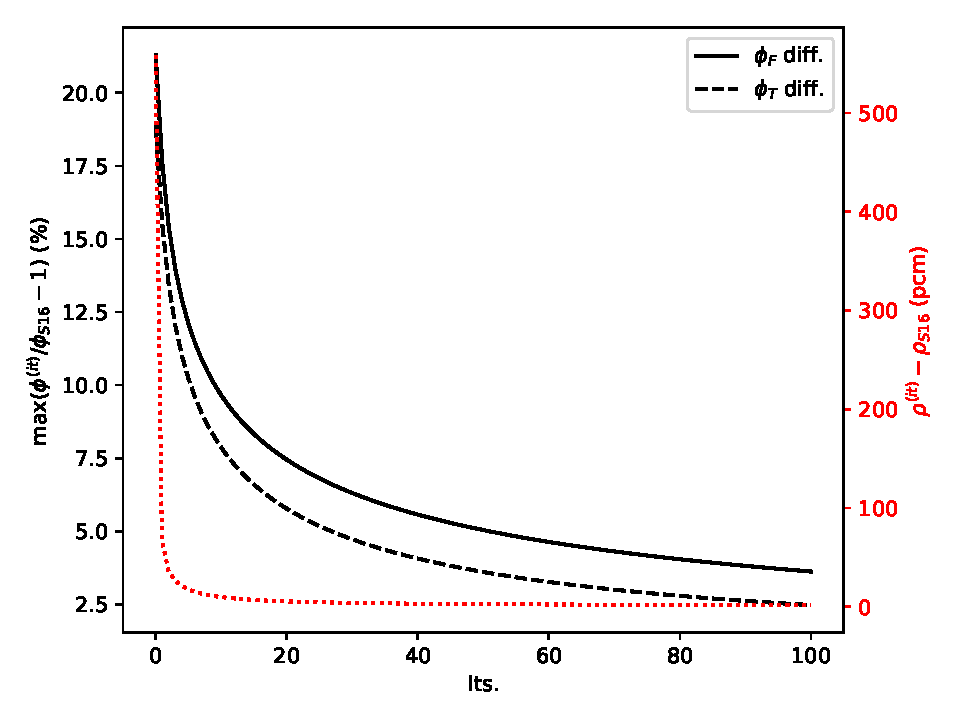
\includegraphics[width=.75\textwidth]{../figures/kflxconv.pdf}
    \caption{Convergence trend.}
  \end{figure}

  \begin{figure}
    \centering
    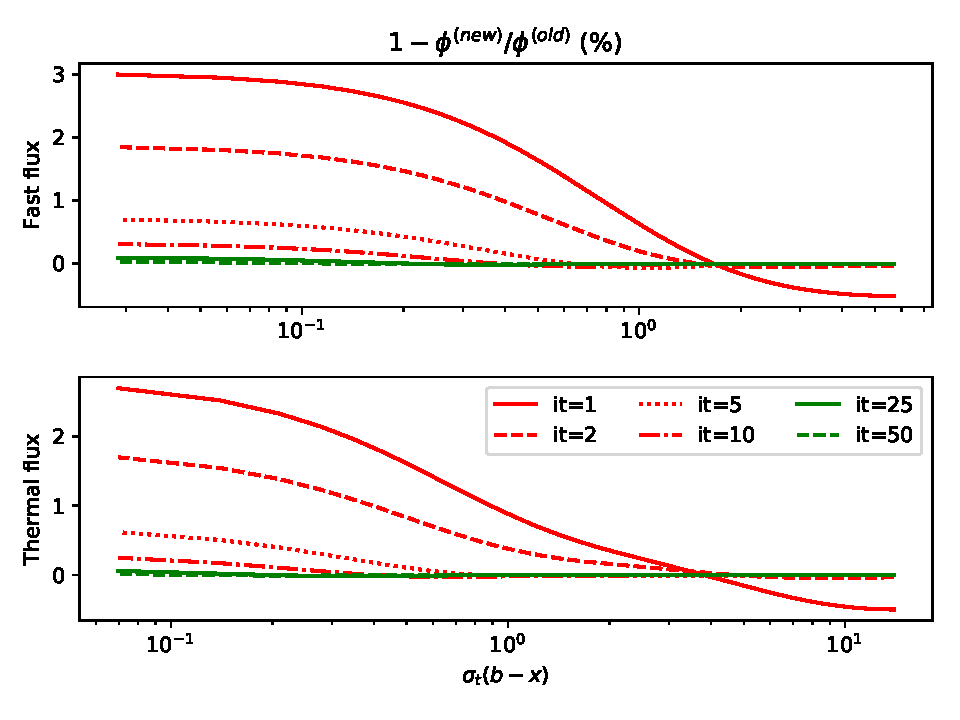
\includegraphics[width=.8\textwidth]{../figures/eflxconv.pdf}
    \caption{Relative flux error in optical lengths from the boundary
             through iterations.}
  \end{figure}

  \begin{exampleblock}{Discussion}\tt
  \begin{itemize}
    \item The Ronen method drives the diffusion solution towards a transport-like solution even with unphysical b.c.
    \item The error concentrates at the boundary interface, and asks for many iterations
    \item $D=1/(3\Sigma_t)$ is the $P_1$ diffusion coefficient here
    \item Although $D=\Sigma_s/(3\Sigma_t^2)$ results in a smaller $\Delta k$, $\Delta \phi$ is 20\% off near the left boundary
  \end{itemize}
  \end{exampleblock}
  \vspace{10mm}

  \begin{alertblock}{Same issues and remarks for multi-dimensional $n$-D cases}\tt
  \begin{itemize}
    \item Can we prove convergence?
    \item Can we compute all components of the diffusion tensor in a coarse mesh?
    \item What are the special functions in $n$-D?
    \item Are there regions (like \emph{void} for instance) where the method cannot be applied?
  \end{itemize}
  \end{alertblock}
\end{frame}

\subsubsection{Curvilinear geometries}
\begin{frame}
  \frametitle{Derivation of the current in 1D curvilinear geometries}
  \vspace{-5mm}
  \begin{columns}
  \column{.5\textwidth}
  {
  Escape probability in \textcolor{ceablue1}{\bf 1D cylindrical geometry}:
  \[
    e_j(r) = \frac{2}{r V_j} \int_0^r { dh\, y \int_{L_j}{
    d \ell \, \text{Ki}_2\left[\tau( y, y - \ell )\right]}},
  \]
  with $y(r, h) = \sqrt{r^2 - h^2}$ and $L_j(h) = [-Y,y] \cap V_j$
  ($Y = y(R, h)$).\\[10mm]
  Escape probability in \textcolor{ceablue1}{\bf 1D spherical geometry}:
  \[
    e_j(r) = \frac{2\pi}{r^2 V_j} \int_0^r { dh\, h y \int_{L_j}{
    d \ell \, \exp\left[-\tau( y, y - \ell )\right]}}.
  \]
  \begin{figure}
    \centering
    \input{../figures/sphere.tkz}
    \caption{Spherical symmetry.}
  \end{figure}
  }
  \column{.5\textwidth}
  \vspace{-10mm}
  \begin{figure}
  \centering
  \scalebox{1.5}{
    \input{../figures/cyltracks.tkz}
  }
  \caption{Tracking integration \cite{hebert2009applied}.}
  \end{figure}
\end{columns}
\end{frame}

%%% %% Introducing the name of ``CEA colors''
%\section{Présentation du style graphique}
%\subsection{Couleurs officielles du CEA}
%\begin{frame}
%  \frametitle{Présentation des couleurs CEA}

%  \begin{center}
%    {\large Implémentées suivant la charte : \textcolor{blue}{\url{http://www-dcom.intra.cea.fr/wp-content/uploads/Logo-regles-applications-charte_CEA-vdef.pdf}} }
%  \end{center}

%  \begin{table}
%    \LARGE
%    \begin{tabular}{l|cccc}
%      Base & & & & \\
%      \hline
%      Rouge & \textcolor{ceared1}{ceared1} & \textcolor{ceared2}{ceared2} & \textcolor{ceared3}{ceared3} & \\
%      Vert & \textcolor{ceagreen1}{ceagreen1} & \textcolor{ceagreen2}{ceagreen2} & \textcolor{ceagreen3}{ceagreen3} & \textcolor{ceagreen4}{ceagreen4} \\
%      Bleu & \textcolor{ceablue1}{ceablue1} & \textcolor{ceablue2}{ceablue2} & \textcolor{ceablue3}{ceablue3} & \\
%      Orange & \textcolor{ceaorange1}{ceaorange1} & \textcolor{ceaorange2}{ceaorange2} & & \\
%      Violet & \textcolor{ceapurple1}{ceapurple1} & \textcolor{ceapurple2}{ceapurple2} & & \\
%      Rose & \textcolor{ceapink1}{ceapink1} & \textcolor{ceapink2}{ceapink2} & & \\

%    \end{tabular}

%  \end{table}

%\end{frame}

%\subsection{Introduction aux raccourcis}
%%% %% Proposed shortcut to create slides
%\theframe{Ce titre de transparent est déjà trop long pour tenir sur une seule ligne}{

%  \begin{itemize}
%  \item Ce slide est fait avec un shortcut pour aller plus vite (voir ``shortcut'')
%  \end{itemize}

%}

%\begin{frame}[allowframebreaks]
%  \frametitle{Test de slide avec allowpagebreak}

%    \begin{block}{Contenu du premier transparent}{
%        \begin{itemize}
%        \item Des choses...
%        \item
%        \item
%        \item
%        \end{itemize}
%      }
%    \end{block}


%  \framebreak

%  \begin{block}{Contenu du second transparent}{
%      \begin{itemize}
%      \item ... et d'autres
%      \end{itemize}
%    }
%  \end{block}

%\end{frame}

%\intercalaire{Titre intercalaire}
%\intercalaireplus{Intercalaire avec du texte}{
%  {\Large Pour dire plus de chose}
%  {\normalsize
%    \begin{itemize}
%    \item Même si c'est pas forcément intéressant
%    \item Même avec des fautes d'orthographe
%    \end{itemize}
%  }
%}

\section{Conclusion}
\theframe{Conclusion}{
%
\begin{exampleblock}{Summary}
%\vspace{3mm}
\begin{itemize} \large
  %\setlength{\itemsep}{3mm}
  \item Diffusion theory is practical for (fast) core calculations
  \item Possible improvements by second-order transport approximations (SP$_N$, A$_N$, \ldots)
  % \item Presentation of transport effects in full core calculation and various diffusive-like transport approximations
  \item The use of \textcolor{ceablue1}{equivalence theory} compensates the lack of physical information in the diffusive model
  \item Introduction of the Ronen Method: principles \& implementation options
  \item Similarities with collision probability methods (see the escape probabilities), without solving CPM, i.e. no matrix inversion
  \item The Ronen Method could provide an \textcolor{ceared1}{online equivalence} between diffusion and integral transport on \textcolor{ceablue1}{coarse meshes}
\end{itemize}
\end{exampleblock}
%\vfill
\begin{alertblock}{Future development}
%\vspace{3mm}
\begin{enumerate}[(i)] \large
  %\setlength{\itemsep}{3mm}
  \item Convergence and stability analysis (using the CMFD scheme)
  \item Formal and numerical investigation of the Ronen Method as a mean for an online equivalence
  % \item Comparison with other deterministic techniques based on integral transport (mainly the collision probability method)
  \item 3D implementation of the Ronen method in nodal codes
  \item Extension to time-dependent problem
\end{enumerate}
\end{alertblock}
}

\section*{References}
\begin{frame}{\insertsectionhead}
%\nocite{*}
\begin{multicols}{2}
\small
\bibliographystyle{plainnat}
\bibliography{RonenMethod}
\end{multicols}
\end{frame}

%% %% Possibility to add a sentence as for intercalaire
\theclosingframe{
  Thanks for your attention!\\[2cm]
  \begin{flushright}\textcolor{white}{
    \visible<2>{
    \emph{Bòja brigant\\[5mm] Ciao Piero!}}
    % \hspace{3cm}
    }
  \end{flushright}
}

%% %% End of main part, beginning of backup (this is used to count the number of slides)
\backupbegin
%% %% New section for backup... the SectionCounter is used (along with totcount) to display at main toc all
%% %% sections but backups
%%\section{Backup}
\setcounter{SectionCounter}{\thesection}
\addtocounter{SectionCounter}{-1}
%% %% Back up menu accessible from any slide where the number of pages is displayed
%%\frame[label=MenuBackup]{\frametitle{Sommaire}
%%  \tableofcontents[sections=\thesection]
%%}

\section*{Other derivation of the diffusion coefficient}
\subsection*{The fundamental leakage model}
\begin{frame}
  \frametitle{The $B_N$ leakage model}
  \begin{alertblock}{Objective}
    Get a critical flux by adjusting the leakage in each group, and obtain a consistent definition of the diffusion coefficient \cite{benoist1964theorie, hebert2009applied}.
  \end{alertblock}
  %
  \begin{block}{Assumptions}
  {
  \begin{itemize} \normalsize
    \item Closed system by \emph{reflective} or \emph{periodic} bnd. conds. in a \textcolor{ceagreen1}{finite lattice of cells or assemblies}.
    \item Flux factorization with a \emph{macroscopic} quantity $\phi$ and a \emph{homogeneous} or \emph{periodic} \textcolor{ceablue1}{fundamental flux} $\psi$, \[\textcolor{ceared1}{\varphi(\mathbf{r}[, \ast]) = \phi(\mathbf{r})\, \psi(\mathbf{r}[, \ast])},\] where $\phi$ fulfills the Helmholtz eqn. $\nabla^2 \phi + B^2 \phi = 0$ with the (\underline{critical}) buckling $B^2 \in \mathbb{R}$. It follows that $\phi \propto \exp(i \mathbf{B} \cdot \mathbf{r})\; (B^2 = \mathbf{B} \cdot \mathbf{B})$.
    \item homogeneous or heterogeneous variants (acc. to the dependence of $\psi$ on $\mathbf{r}$)
  \end{itemize}
  }
  \end{block}
  %
  \begin{exampleblock}{Homogeneous $B_1$ Equations}
  {
  After a flux-volume homogenization of the NTE, substitute $\varphi = \psi(E, \bOm)\exp(i \mathbf{B} \cdot \mathbf{r})$ and integrate on angle to obtain the system of eqs. (with $\gamma$ as polynomial function of $(B/\Sigma_t)^2$):
  %\[ \left\{ \begin{split}
  \begin{align*}[left=\empheqlbrace]
    (\Sigma_t(E) + D(B, E)B^2) \psi(E) = \int_{0}^{\infty}{dE' \left(\Sigma_{s,0}(E' \rightarrow E) + \chi(E) \nu\Sigma_f(E') \right)\psi(E')}\\
    \textcolor{ceared1}{
    D(B, E) = \frac{1}{3\gamma(B, \Sigma_t)\Sigma_t}\left[ 1 + 3\int_{0}^{\infty} {dE' \Sigma_{s,1}(E' \rightarrow E) D(B, E') \frac{\psi(E')}{\psi(E)}} \right]}
  \end{align*}
  %\end{split} \right. \]
  }
  \end{exampleblock}
\end{frame}

\subsection*{Diffusive-like approximations from radiative transfer}
\begin{frame}
  \frametitle{Other diffusive-like approximations from radiative transfer problems}
  \begin{block}{Flux-limited diffusion}
  {
  The angular flux is factored in a term slowly varying in space and a normalized angular component \cite{levermore1981flux}:
  \[
  \varphi \approx \phi(\mathbf{r}, E) \psi(\mathbf{r}, \bOm) \quad \text{with} \quad \int_{4\pi} {d \bOm \psi} = 1,
  \quad \implies \mathbf{J}_g = \mathbf{f}(\mathbf{r})\,\phi_g \; \wedge \;
  \frac{\lVert \mathbf{J}_g \rVert}{\phi_g} = \text{const},\; \forall g.
  \]
  The diffusion coefficient (``the flux-limiting parameter'') come from the solution of a \emph{transcendental equation}. In the limit of weak gradients, the diffusion coefficient is obtained as (for all groups):
  \[ \textcolor{ceared1}{
  D_g(\mathbf{r}) = \frac{1}{3} \left[ \Sigma_{t,g} - \sum_{g'}{\Sigma_{s,1,g' \rightarrow g} \,\frac{\phi_{g'}}{\phi_g}} \right]^{-1}}
  \]
  }
  \end{block}
  %
  \begin{block}{Variable Eddington factor}
  {
  Postulate a factorization of the second moment by another factor (or \emph{tensor}) slowly varying in space \cite{pomraning1982flux}:
  \[
  \varphi \approx E(\mathbf{r}[, \ast]) \phi(\mathbf{r}[, \ast]),
  \text{ and }
  \partial_{\mathbf{r}} E \approx 0 \hfill \implies
  \textcolor{ceared1}{
  D_{i,g}(\mathbf{r}) = E_g(\mathbf{r}) \left[ \Sigma_{t,g} - \sum_{g'}{\Sigma_{s,1,g' \rightarrow g} \,\frac{J_{i,g'}}{J_{i,g}}} \right]^{-1}, i \in (\hat{e}_x, \hat{e}_y, \hat{e}_z).}
  \]
  }
  \end{block}
\end{frame}

\subsection*{Homogenization and Equivalence Theory}
\begin{frame}
  \frametitle{Homogenization and Equivalence Theory}
  %
  \begin{block}{} \begin{flushright}
  \textcolor{ceared1}{\Large What for?} Prepare \emph{in advance} all reactor data for later core calculations in \textcolor{ceablue1}{low-order transport} (diffusion, $SP_N$ and others). \end{flushright}
  \end{block}\vspace{5mm}
  %
  \begin{alertblock}{Main rational of Homogenization}
    Conservation of reaction rates in the volume $\mathcal{V}$ of
    \emph{spatial homogenization} and
    in the $g$-th group of \emph{energy condensation} with
    $E \in [E_g, E_{g+1}]$, $g = 1, \ldots, G$.
  \end{alertblock}
  %
  \[
  \Sigma_g = \frac{\displaystyle
    \int_{\mathcal{V}} d\mathbf{r} \int_{E_{g+1}}^{E_g} dE \,
      \Sigma(\mathbf{r}, E) \, \phi(\mathbf{r}, E) }{\displaystyle
    \int_{\mathcal{V}} d\mathbf{r} \int_{E_{g+1}}^{E_g} dE \, \phi(\mathbf{r}, E)
    } \quad \text{with} \quad \chi_g = \int_{E_{g+1}}^{E_g} dE \, \chi(E).
  \]
  %
  \begin{columns}
    \column{.6\textwidth}
      \begin{block}{Equivalence}
      \textcolor{ceared1}{\Large Why?} $\ldots$Diffusion $\not\equiv$ transport, conservation of reaction rates does not imply to reproduce the \emph{same currents} at the boundaries of $\mathcal{V}$. Available techniques:
      \begin{itemize}
        \item (A)DF$ = \phi_{\text{het}}/\phi_{\text{hom}} $ (discontinuity factors), \emph{two per direction}
        \item SPH (SuPer-Homogenization) factors, \emph{one per group and homog. region}: $(\Sigma^{(k)}_g / s)(s\phi^{(k)}_g)$
      \end{itemize}
    \end{block}
    %
    \column{.4\textwidth} \centering
    \def\wdt{2.5}
    \def\ymin{0.25}
    \begin{tikzpicture}
      \draw[->, thin, help lines] ({-\wdt-0.5},{\ymin+0.1})
        -- ({\wdt+1},{\ymin+0.1}) node[right] {$\hat{e}_k$};
      \draw[-] (-\wdt,\ymin) node[below] {$k-1/2$} -- (-\wdt,3);
      \draw[-] ({\wdt-1/4},\ymin) node[below] {$k+1/2$} -- ({\wdt-1/4},3);
      \draw[->] ({-\wdt-0.5}, 2.4) -- ({-\wdt-0.1}, 2.4)
        node[midway,above] {$J^+_{\text{in}}$};
      \draw[black, domain={-\wdt}:{\wdt-1/4}]
        plot[samples=100]
        ({\x}, {2+0.2*sin(((\x+2)*4)*3.141592 r)-0.2*\x})
        node[right] {$\phi_{\text{het}}$};
      \draw[red, domain={-\wdt}:{\wdt-1/4}, thick]
        plot[samples=100] ({\x}, {0.5+exp(-0.35*\x)})
        node[right] {$\phi_{\text{hom}}$};
      \node[red,below] (D) at (\ymin,1.35) {$D^{(k)}$};
      \node (title) at (0,3) {$k$'th cell};
    \end{tikzpicture}
  \end{columns}
\end{frame}

\subsection*{Special functions}

\begin{frame}
  \frametitle{\insertsubsectionhead}
  {
  Integral exponential function E$_n$:
  \[
    E_n(\tau) = \int_1^{\infty}{du\, \frac{e^{-|tau|\,u}}{u^n}}
      = \int_0^1 {d\mu \, \mu^{n-2} e^{-|\tau| / \mu}}.
  \]
  Useful properties: $d_{\tau} \text{E}_n = -\text{E}_{n-1}(\tau)$ and
  $\text{E}_n(0)={frac{1}{n+1}}$.
  \vspace{10mm}
  Bickley-Naylor functions Ki$_n$:
  \[
    \text{Ki}_n(\tau) = \int_0^{\pi/2}{ d\theta \sin^{n-1} \theta \exp\left(-\frac{\tau}{\sin \theta}\right) }.
  \]
  Useful properties: $d_{\tau} \text{Ki}_n = -\text{Ki}_{n-1}(\tau)$.
  }
\end{frame}


%% %% End of backup mode....
\backupend

\end{document}
